% !TeX root = ../main.tex

\chapter{简介}

\section{研究背景和意义}

地表形变的监测是了解地球内部物理过程的重要手段。
许多地球物理现象,如火山,地震等,都会伴随地表的形变。
地表形变携带着这些现象的信息,如果能够正确地提取并使用这些信息,
会加深人类对于地球表面及内部各种物理化学演化过程的了解,
更好地服务于社会的生产和生活。

在实际应用中,地表形变的监测是了解和预防地质灾害的重要方法。
近年来,地面沉降及其引发的次生灾害对各国的经济及社会发展造成越来越严重的损失。
然而,传统的形变监测手段难以满足当前监测的要求:
传统方法需要人工在有限的点上布设台站,需要人力长期参与,且某些条件恶劣的区域很难人工操作;
由于人力成本的限制,在大尺度的范围上很难布设足够密的台站,而过于稀疏的台站并不能满足监测的需求。

合成干涉孔径雷达(Interferometric Synthetic Aperture Radar,InSAR)监测
具有成本低,覆盖范围广,全天候,非接触等优良特点。
而且相较于GPS,InSAR在垂直方向的能提供更高的精度,%\cite{knuth84}
目前已在地表沉降监测方面广泛应用,且取得了突出的成果
\cite{kimEvolutionSinkholesWink2019b,shiSubsidenceSinkholesWink2019a}。

本文通过研究一卤水井的沉降,验证了InSAR技术在研究此类现象上的有效性,
并对该区域的沉降建立物理模型,
所得的物理模型和实际导致沉降的地下空洞一致性良好,
进一步地表明InSAR技术在此类问题确实是一种有效的办法,
并且成本较低,值得我国大力推广。

\section{国内外研究现状}
由于InSAR技术在地表形变监测领域的独特优势,
在它从诞生开始受到微波遥感领域的强烈关注。
近些年来,InSAR发展出来一系列的算法,如PS(persistent scatterer)
\cite{ferrettiPermanentScatterersSAR2001,hooperNewMethodMeasuring2004},
SBAS(small baseline subsets)
\cite{berardinoNewAlgorithmSurface2002,hooperMultitemporalInSARMethod2008},
SqueeSAR\cite{ferrettiNewAlgorithmProcessing2011}
等,
能够对克服原始InSAR技术的种种劣势,
在地表形变监测领域有广泛的应用。

在1978年NASA SEASET卫星发射以后,星载SAR开始登上历史舞台并应用与地球表面研究。
关于星载干涉SAR的原理研究最早可以追溯到20世纪70年代\cite{ziskNewEarthbasedRadar1972},
InSAR的首次应用发生在上个世纪80年代末
\cite{zebkerTopographicMappingInterferometric1986,goldsteinInterferometricRadarMeasurement1987}。
1989年,Gabriel首次使用D-InSAR技术验证了InSAR技术可以在大尺度(50km)区域上检测到极小的形变(1cm或更小)
\cite{gabrielMappingSmallElevation1989},
验证了InSAR技术在沉降监测方面的可行性。

2001年,Ferretti等人首次提出PS-InSAR技术(permanent scatterer)
\cite{ferrettiPermanentScatterersSAR2001}
并将其应用与地面沉降速率的监测
\cite{ferrettiNonlinearSubsidenceRate2000}。
2004年,Hooper提出了新的PS-InSAR算法(persistent scatterer),
并将这一新的算法应用于植被茂盛的火山区域,获取了地表的形变速率
\cite{hooperNewMethodMeasuring2004},
对比发现,此PS算法的结果和GPS与水准测量的结果吻合,
大部分的PS点的可靠性较高。
2008年,Hooper将PS-InSAR和SBAS结合,
提取了更多的PS点,并进一步提高了信噪比
\cite{hooperMultitemporalInSARMethod2008}。
2011年,Ferretti等人将PS点(persistent scatterer)和DS点(distributed scatterer)
的信号结合,提出了SqueeSAR技术。

自从1991年ERS-1卫星发射,大量的SAR数据被获取,使得InSAR得到了广泛的应用。
目前InSAR技术的应用主要分为以下几个方面:
\begin{enumerate}
  \item 火山的喷发期和休眠期地表的形变可以用来研究火山结构,
  火山喷发机制,以及做火山灾害的危害性评估\cite{luInSARImagingVolcanic2007};
  \item 地震震前,震时,震后的地表形变提供了震源定位,断层几何形状,岩石破裂动力学过程;
  地壳和上地幔物理性质等研究的必要信息
  \cite{massonnetDisplacementFieldLanders1993,biggsMultiinterferogramMethodMeasuring2007};
  \item 地下水的注入和开采,矿物开采,缓慢移动的滑坡导致的形变能够为此类现象的负面性影响的评估和缓解提供数据支持
  \cite{zhangMappingGroundSurface2012,zhaoLargeareaLandslideDetection2012};
  \item 冰川移动的数据能提高人类对全球变暖以及海平面上升的认识
  \cite{rignotMassBalancePolar2002};
  \item 湿地水平面的变化可以提高对洪水灾害的认识和评估
  \cite{luRadarsat1ERSInSAR2008}。
\end{enumerate}

\section{本研究的主要内容}

\subsection{使用SBAS-InSAR技术获取当地地表形变}
本研究选取该卤水井所在区域(约1km×1km)ALOS 1(Advanced Land Observation Satellite 1)从2007年到2011年的15幅影像,
通过SBAS-InSAR技术获取当地地表形变以及平均的形变速率。这一步使用的软件为StamPS。


\subsection{使用mogi模型对该形变建模}
首先观察SBAS-InSAR得到的形变特征,选取比较合适的mogi模型,对该形变进行理论建模,
建模所使用的软件为GBIS。
然后与已有的研究成果相对比,并结合当地地质背景,分析所得模型的可靠程度。

本研究的组织结构如图\ref{fig:flow}所示。
\begin{figure}[htb]
  \centering
  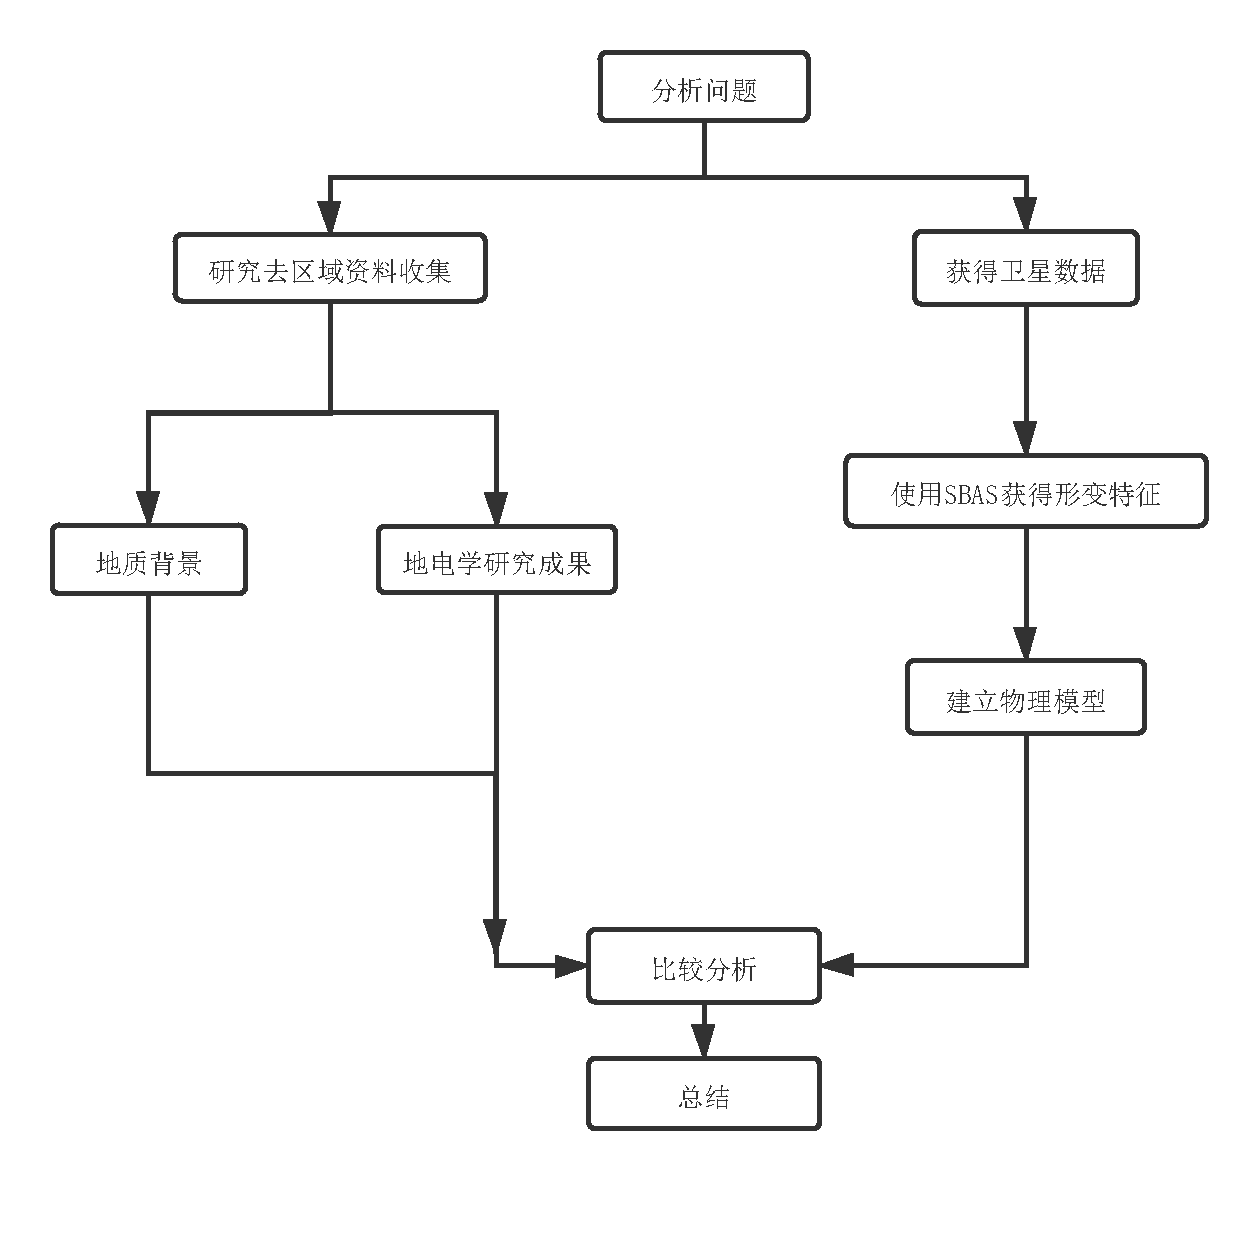
\includegraphics[width=\textwidth]{flow.pdf}
  \caption{本研究的组织结构}
  \label{fig:flow}
\end{figure}